\documentclass[tikz,border=8pt]{standalone}

\usepackage{garamondx}

\usepackage{xcolor}
\usepackage{varwidth}

\usepackage{tikz}
\usetikzlibrary{calc,arrows.meta,positioning,fit,shapes,shapes.geometric,arrows,tikzmark,backgrounds}

\definecolor{darkolivegreen}{rgb}{0.33, 0.42, 0.18}
\definecolor{darkbyzantium}{rgb}{0.36, 0.22, 0.33}
\definecolor{darkelectricblue}{rgb}{0.33, 0.41, 0.47}
\definecolor{deepchestnut}{rgb}{0.73, 0.31, 0.28}

\tikzstyle{background}=[rectangle, rounded corners, minimum width=7em, minimum height=2em, text centered, draw=black, fill=deepchestnut!30, text width=7em]
\tikzstyle{psych}=[rectangle, rounded corners, minimum width=10em, minimum height=2em, text centered, draw=black, fill=darkelectricblue!30, text width=7em]
\tikzstyle{node}=[minimum width=7em, minimum height=2em, text centered, text width=7em]
\tikzstyle{arrow}=[very thick, ->, >=latex]
\tikzstyle{arrow'}=[very thick, <->, >=stealth]

\pgfdeclarelayer{background}
\pgfdeclarelayer{foreground}
\pgfsetlayers{background,main,foreground}

\begin{document}
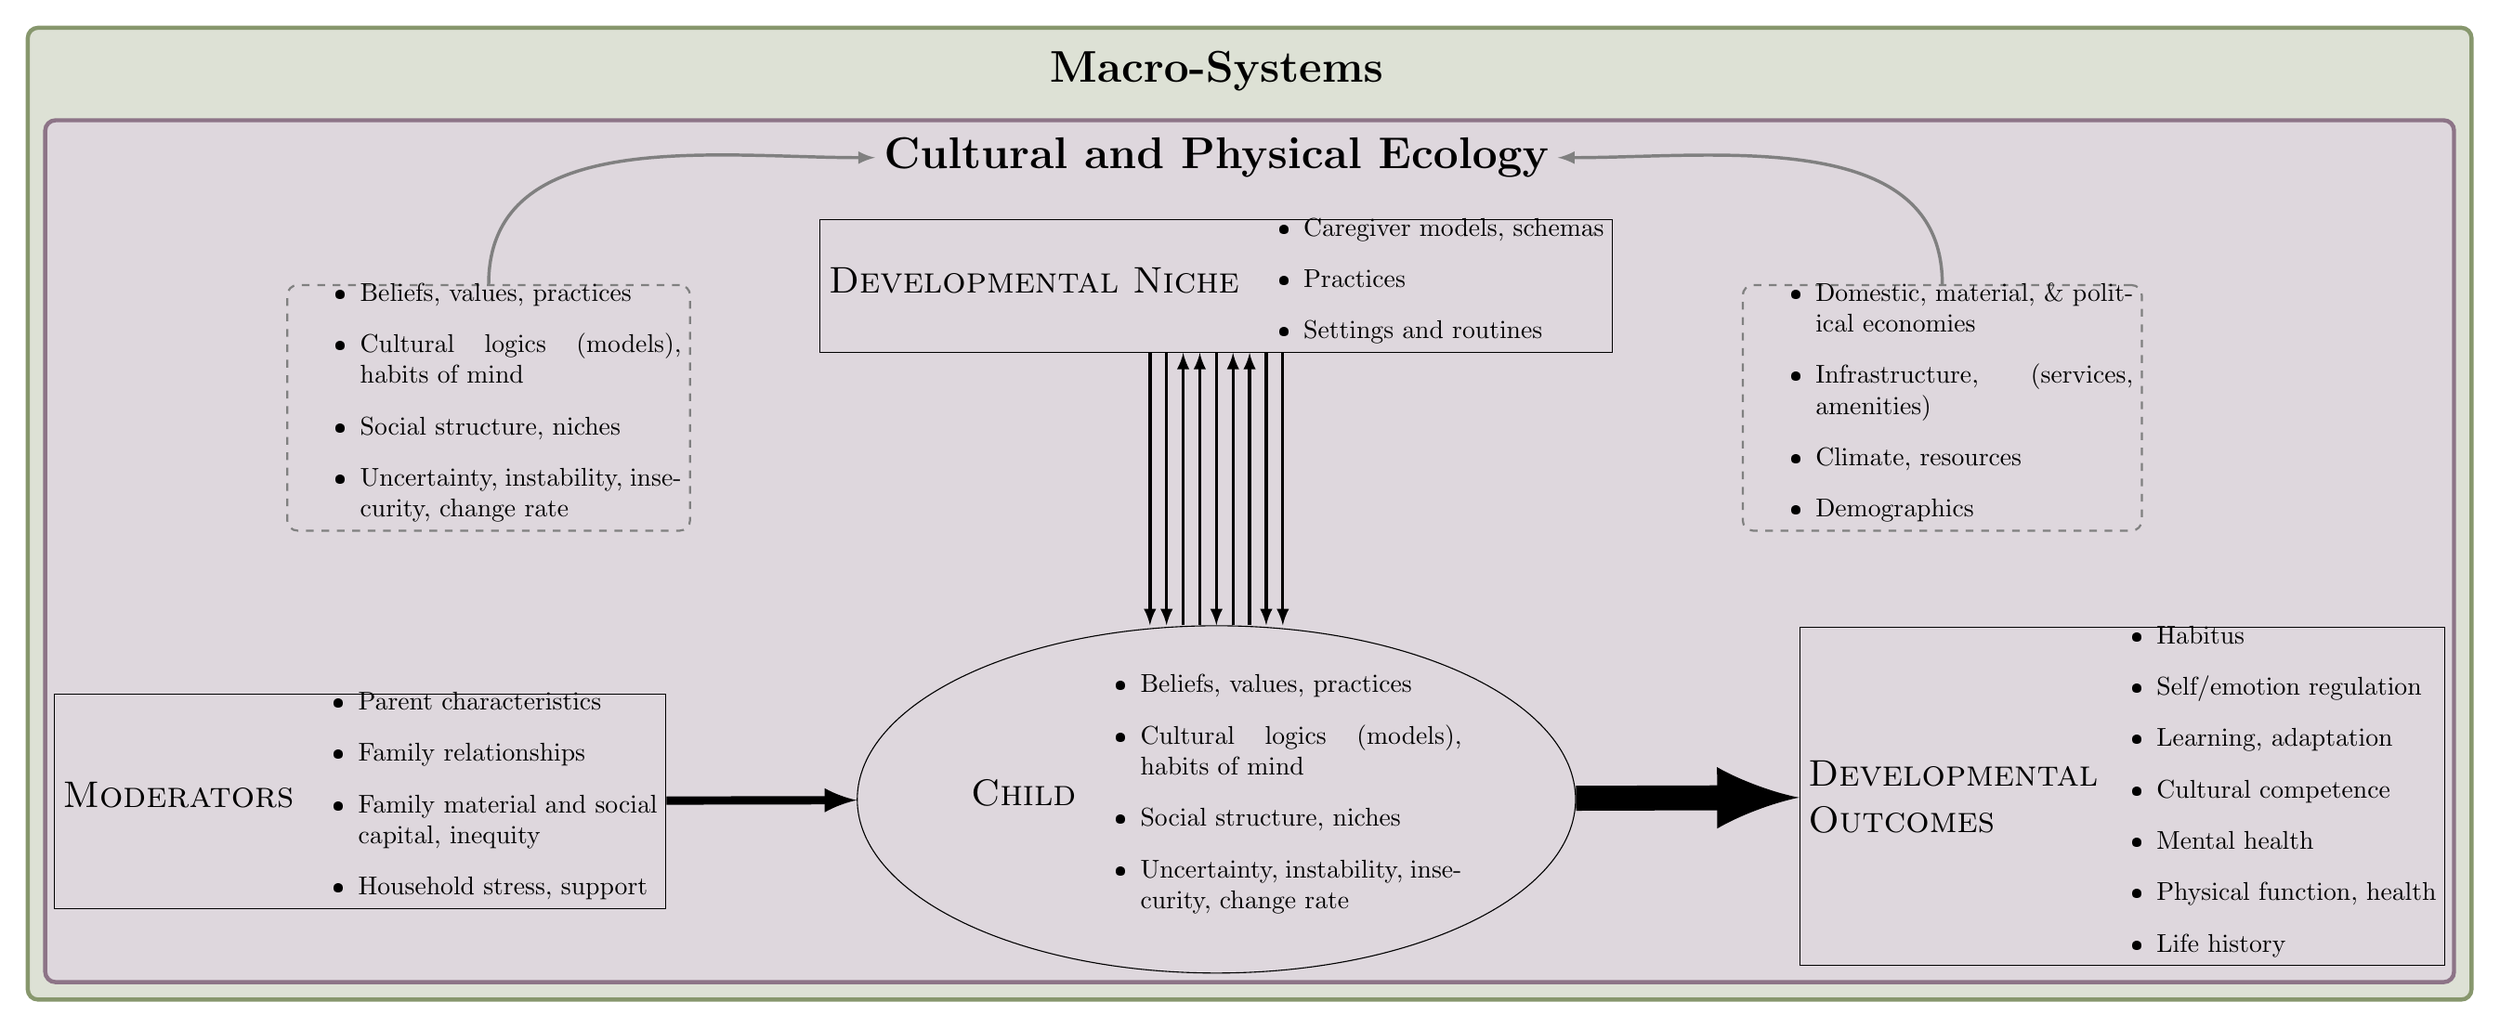
\begin{tikzpicture}[node distance=5em]

\begin{pgfonlayer}{foreground}
	\node[minimum width=7em,text centered](macro){\LARGE\scshape\bfseries Macro-Systems};
	\node[minimum width=7em,text centered,yshift=9ex](ecol)[below=of macro] {\LARGE\scshape\bfseries Cultural and Physical Ecology};
	\node[minimum width=7em,text centered,draw=black, text=black](devn) [below of=ecol]{\textsc{\Large Developmental Niche}\begin{varwidth}{15em}\begin{itemize}
		\item Caregiver models, schemas
		\item Practices
		\item Settings and routines
		\end{itemize}\end{varwidth}};
	\node[minimum width=7em,text centered,draw=gray, dashed, rounded corners, left=of devn, text=black, thick, yshift=-11ex](a1){\begin{varwidth}{15em}\begin{itemize}
		\item Beliefs, values, practices
		\item Cultural logics (models), habits of mind
		\item Social structure, niches
		\item Uncertainty, instability, insecurity, change rate
		\end{itemize}\end{varwidth}};
	\node[minimum width=7em,text centered, draw=gray, dashed, rounded corners, right=of devn, text=black, thick, yshift=-11ex](a2){\begin{varwidth}{15em}\begin{itemize}
		\item Domestic, material, \& political economies
		\item Infrastructure, (services, amenities)
		\item Climate, resources
		\item Demographics
		\end{itemize}\end{varwidth}};
	\node[minimum width=7em,text centered,draw=black, ellipse, below=of devn,yshift=-13ex](child){\textsc{\Large Child}\\\begin{varwidth}{15em}\begin{itemize}
		\item Beliefs, values, practices
		\item Cultural logics (models), habits of mind
		\item Social structure, niches
		\item Uncertainty, instability, insecurity, change rate
		\end{itemize}\end{varwidth}};
	\node[minimum width=7em,text centered,draw=black, below=of a1,xshift=-5em,yshift=-3ex](mod){\textsc{\Large Moderators}\begin{varwidth}{15em}\begin{itemize}
		\item Parent characteristics
		\item Family relationships 
		\item Family material and social capital, inequity
		\item Household stress, support
		\end{itemize}\end{varwidth}};
	\node[minimum width=7em,text centered,draw=black, below=of a2,xshift=7em,yshift=3ex](devo){\textsc{\begin{varwidth}{10em}\Large Developmental Outcomes\end{varwidth}}\begin{varwidth}{15em}\begin{itemize}
		\item Habitus
		\item Self/emotion regulation
		\item Learning, adaptation
		\item Cultural competence
		\item Mental health
		\item Physical function, health
		\item Life history
		\end{itemize}\end{varwidth}};
	
	\draw[arrow,line width=0.125em,draw=gray] (a1) to [out=90,in=180] (ecol);
	\draw[arrow,line width=0.125em,draw=gray] (a2) to [out=90,in=0] (ecol);
	\draw[arrow,line width=0.75ex](mod) to (child);
	\draw[arrow,line width=2.25ex](child) to (devo);
	\draw[arrow,transform canvas={xshift=-6ex}] (devn) -- (child);
	\draw[arrow,transform canvas={xshift=-4.5ex}] (devn) -- (child);
	\draw[arrow,transform canvas={xshift=-3ex}] (child) -- (devn);
	\draw[arrow,transform canvas={xshift=-1.5ex}] (child) -- (devn);
	\draw[arrow] (devn) -- (child);
	\draw[arrow,transform canvas={xshift=1.5ex}] (child) -- (devn);
	\draw[arrow,transform canvas={xshift=3ex}] (child) -- (devn);
	\draw[arrow,transform canvas={xshift=4.5ex}] (devn) -- (child);
	\draw[arrow,transform canvas={xshift=6ex}] (devn) -- (child);
\end{pgfonlayer}


\begin{scope}[in front of path]
  \node [fit=(ecol) (devn) (a1) (a2) (mod) (child) (devo),draw=darkbyzantium!70,fill=darkbyzantium!20,behind path,ultra thick,rounded corners] {};
\end{scope}

\begin{pgfonlayer}{background}
  \draw[draw=darkolivegreen!70,fill=darkolivegreen!20,ultra thick,rounded corners] ($(current bounding box.south east)+(6pt,-6pt)$) rectangle ($(current bounding box.north west)+(-6pt,6pt)$);
\end{pgfonlayer}

\end{tikzpicture}

\end{document}
